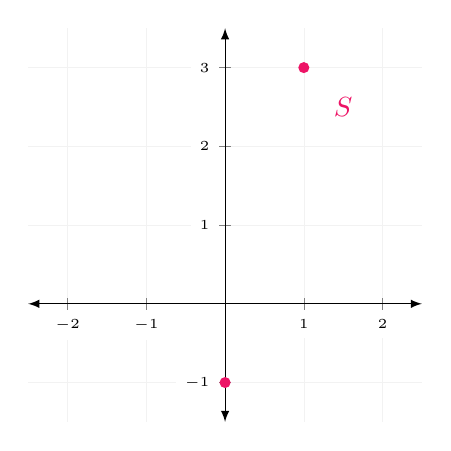
\begin{tikzpicture}[baseline = (current bounding box.north)]
				\begin{axis}[
					anchor=origin,
					disabledatascaling,
					xmin=-2,xmax=2,
					ymin=-1,ymax=3,
					xtick={-2,...,2},
					ytick={-1,...,3},
					x=1cm,y=1cm,
					grid=both,
					grid style={line width=.1pt, draw=gray!10},
					axis lines=middle,
					minor tick num=0,
					enlargelimits={abs=0.5},
					axis line style={latex-latex},
					ticklabel style={font=\tiny,fill=white},
					xlabel style={at={(ticklabel* cs:1)},anchor=north west},
					ylabel style={at={(ticklabel* cs:1)},anchor=south west}
				]
					\fill [WildStrawberry] (1,3) circle[radius=2pt];
					\fill [WildStrawberry] (0,-1) circle[radius=2pt];
				\end{axis}
				\node [WildStrawberry] at (1.5,2.5) {$S$};
			\end{tikzpicture}
